\documentclass[10pt,a4paper,final]{article}
%
\usepackage[utf8x]{inputenc}
\usepackage{ucs}
\usepackage{amsmath}
\usepackage{geometry}
\usepackage{anysize} % Soporte para el comando \marginsize
\usepackage{graphicx}
\usepackage{amsfonts}
\usepackage{amssymb}
\usepackage[spanish]{babel}
%%%%%%%%%%%%%%%%%%%%%%%%%%%%%%%%%%%%%%%%%%%%%%%%%
%%%%%%%%%%%%%%%%%%%%%%%%%%%%%%%%%%%%%%%%%%%%%%%%%
%%%%%%%%%%%%%%%%%%%%%%%%%%%%%%%%%%%%%%%%%%%%%%%%%
\marginsize{2cm}{2cm}{1.5cm}{1.5cm}
%
\begin{document}
\title{Calculo de descensos en un campo de bombeo en medios porosos}
\author{Christian N. Pfarher, Juan Pablo Garbarino, Marina Castro\\
\textit{Trabajo práctico final de ``Métodos numéricos y simulación'', II-FICH-UNL.}}
\markboth{Método numérico y simulación: TRABAJO FINAL}{}
\date{\today}
\maketitle
%%%%%%%%%%%%%%%%%%%%%%%%%%%%%%%%%%%%%%%%%%%%%%%%%
%%%%%%%%%%%%%%%%%%%%%%%%%%%%%%%%%%%%%%%%%%%%%%%%%
%%%%%%%%%%%%%%%%%%%%%%%%%%%%%%%%%%%%%%%%%%%%%%%%%
\newpage
\tableofcontents
%%%%%%%%%%%%%%%%%%%%%%%%%%%%%%%%%%%%%%%%%%%%%%%%%
%%%%%%%%%%%%%%%%%%%%%%%%%%%%%%%%%%%%%%%%%%%%%%%%%
%%%%%%%%%%%%%%%%%%%%%%%%%%%%%%%%%%%%%%%%%%%%%%%%%
\newpage
%%%%%%%%%%%%%%%%%%%%%%%%%%%%%%%%%%%%%%%%%%%%%%%%%
%%%%%%%%%%%%%%%%%%%%%%%%%%%%%%%%%%%%%%%%%%%%%%%%%
%%%%%%%%%%%%%%%%%%%%%%%%%%%%%%%%%%%%%%%%%%%%%%%%%
\section{Introducción}
En el presente trabajo, se presentan los resultados de la simulación de un campo de bombeo en medios porosos. El campo
consta de 2 pozos de bombeo de agua que funcionan por 15 horas seguidas. 

Para la realización del trabajo se utilizó el software de pre y pos proceso GiD \footnote{http://gid.cimne.upc.es/}. Mediante el mismo, se utilizó el \emph{módulo de pre-proceso} para la carga de los datos del problema, mientras que para
la simulación se utilizó Tdyn \footnote{es un entorno tridimensional de análisis fluidodinámico (CFD) y multifísica basado en el método de los elementos finitos estabilizado}(\emph{módulo de post-proceso}).
%%%%%%%%%%%%%%%%%%%%%%%%%%%%%%%%%%%%%%%%%%%%%%%%%
%%%%%%%%%%%%%%%%%%%%%%%%%%%%%%%%%%%%%%%%%%%%%%%%%
%%%%%%%%%%%%%%%%%%%%%%%%%%%%%%%%%%%%%%%%%%%%%%%%%
\section{Objetivos}
El objetivo de este trabajo, consiste en la simulación de lineas de corrientes y equipotenciales en un campo de bombeo (medio poroso) con 2 bombas de extracción de agua en un acuífero libre (no confinado), homogéneo e isótropo.

%%%%%%%%%%%%%%%%%%%%%%%%%%%%%%%%%%%%%%%%%%%%%%%%%
%%%%%%%%%%%%%%%%%%%%%%%%%%%%%%%%%%%%%%%%%%%%%%%%%
%%%%%%%%%%%%%%%%%%%%%%%%%%%%%%%%%%%%%%%%%%%%%%%%%
\section{Base Teórica}
básicamente es la ecuación de poisson con k
representado la permeabilidad.
\subsection{Modelo matemático o fisico.. ver}
describir mod mate.
 son las ecuaciones matemáticas, en nuestro caso las
ecuaciones de navier stokes
%
\subsection{Modelo numérico}
describir mod num.
tdyn resuelve en el espacio por el método de
elementos finitos y temporalmente hay que fijarse que opción está
tildada.
%%%%%%%%%%%%%%%%%%%%%%%%%%%%%%%%%%%%%%%%%%%%%%%%%
%%%%%%%%%%%%%%%%%%%%%%%%%%%%%%%%%%%%%%%%%%%%%%%%%
%%%%%%%%%%%%%%%%%%%%%%%%%%%%%%%%%%%%%%%%%%%%%%%%%
\section{Desarrollo}
\subsection{Datos del problema}
Los datos que se pudieron obtener del problema son:
\begin{itemize}
	\item Discretización del área a modelar:	
	\begin{itemize}
		\item Dominio: $x=1000 ~m.$, $y=1000 ~m.$
		\item Acuífero libre, homogéneo e isótropo $(K_x = K_y = K_z)$
		\item Espesor del acuífero: $20 ~m.$
	\end{itemize}
	%
	\item Ubicación de los Pozos de bombeo:
	\begin{itemize}
		\item Pozo Bombeo 1: $x=150~m.$, $y=650 ~m.$
		\item Pozo Bombeo 2: $x=750~m.$, $y=250 ~m.$
	\end{itemize}
	%
	\item Caudal de bombeo:
	\begin{itemize}
		\item Pozo Bombeo 1: $60~m³/h$
		\item Pozo Bombeo 2: $40~m³/h$
		\item[] Ambos posos trabajan 15 horas por día
	\end{itemize}
	\item Filtro: Tramo filtrante de $150~m.$ de longitud
	\item Transmisividad: $600~m²/d$
	\item Porosidad efectiva: $5*10⁻²$
\end{itemize}
%
\subsection{Definición de Geometría}
Para la geometría en tres dimensiones se tiene los siguientes datos:
En las figuras \ref{cotas_superiores_generalesXY}, \ref{cotas_superiores_detallesXY} y \ref{cotas_grales_YZ} se pueden observar
las dimensiones de las geometrías según los datos del problema. Hay que aclarar aquí que el cuadrado de $300~m.~x~300~m.$ que se visualiza
en la figura \ref{cotas_superiores_detallesXY} como el rectángulo de $400~m.~x~300~m.$ en la misma figura, solo fueron dibujados con el
objetivo, de a posteriori, realizar un refinamiento del dominio en la zona que más intereza visualizar.\\
***************************
aclarara aca lo de los redimensioneamientos y demas...
***************************
\begin{figure}[tbhp]
\centerline{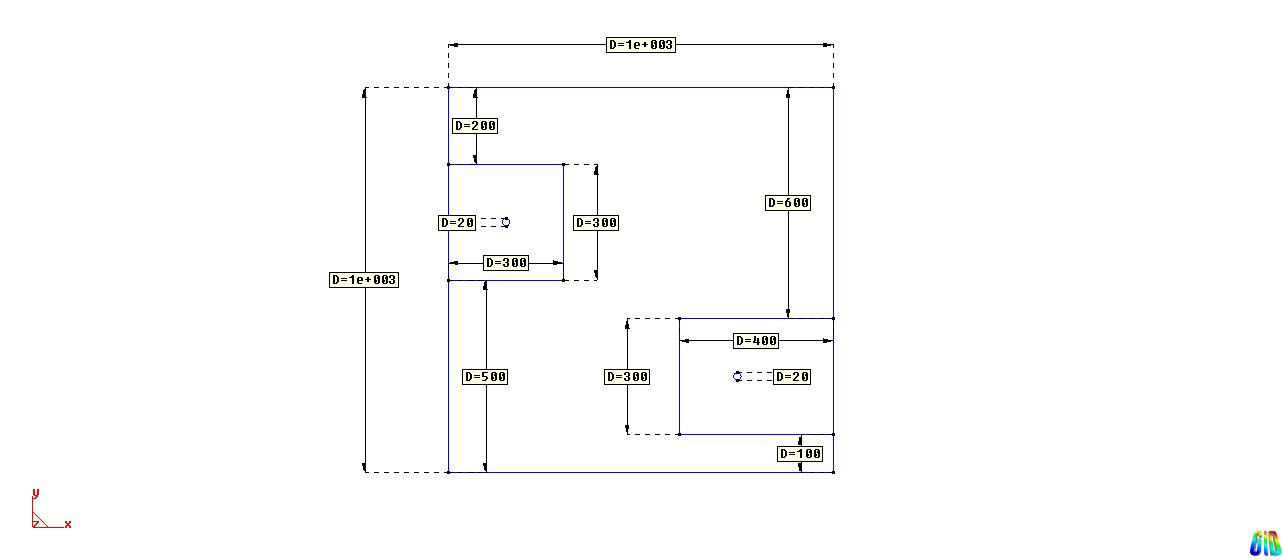
\includegraphics[scale=0.75]{img/cotas_superiores_generalesXY}}
\caption{Vista General de las cotas en el Plano XY}
\label{cotas_superiores_generalesXY}
\end{figure}

%
\begin{figure}[tbhp]
\centerline{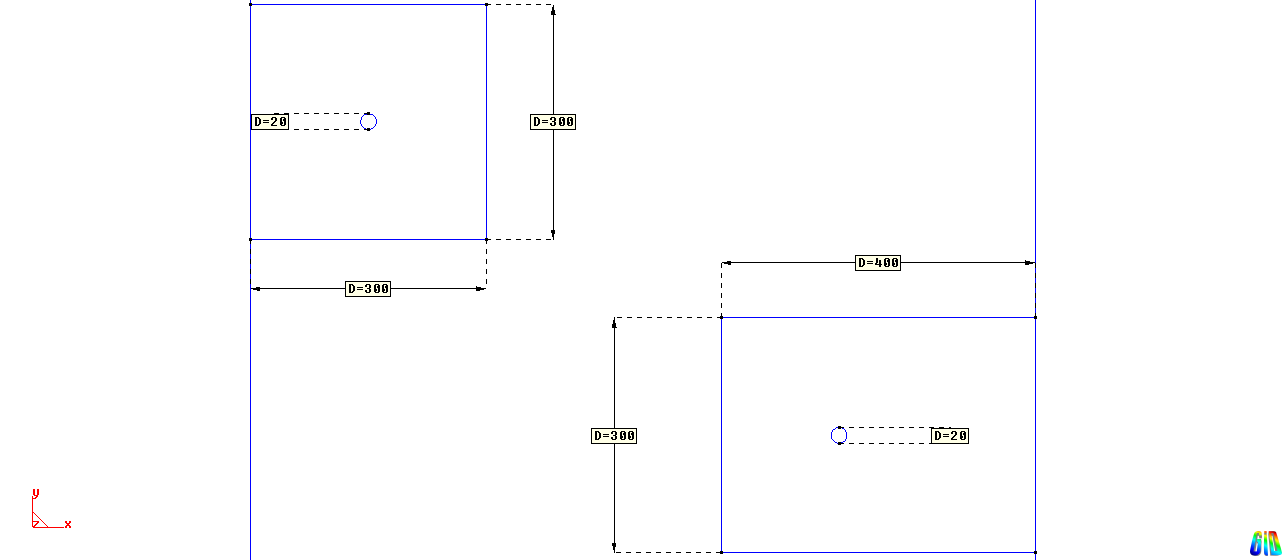
\includegraphics[scale=0.75]{img/cotas_superiores_detallesXY}}
\caption{Vista en detalle (pozos) de las cotas en el Plano XY}
\label{cotas_superiores_detallesXY}
\end{figure}
%

%
\begin{figure}[tbhp]
\centerline{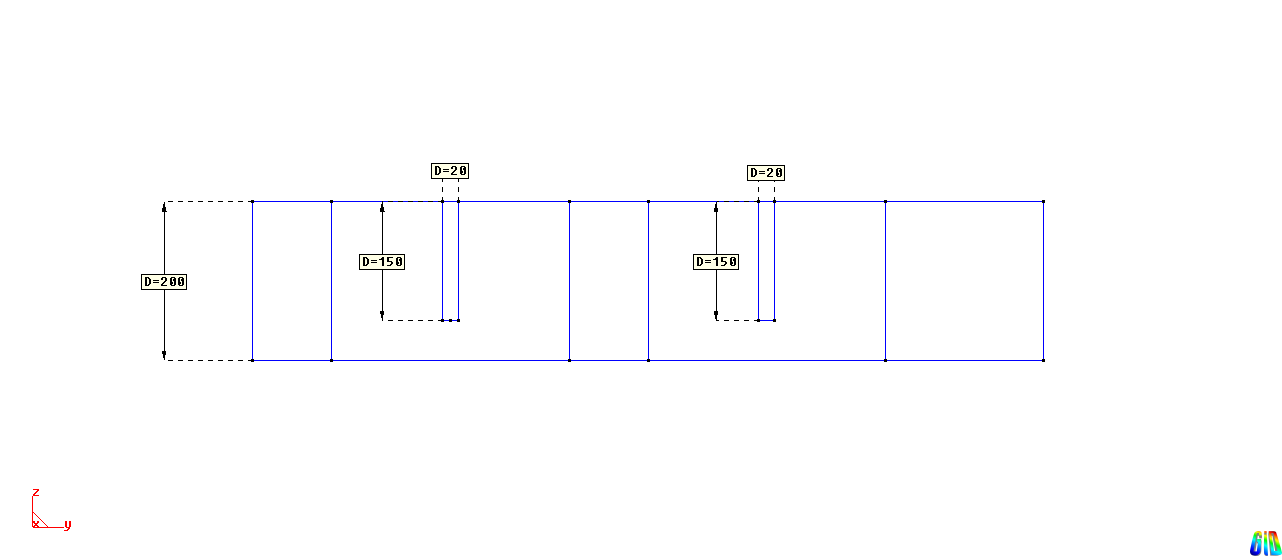
\includegraphics[scale=0.75]{img/cotas_grales_YZ}}
\caption{Vista en de las cotas en el plano YZ}
\label{cotas_grales_YZ}
\end{figure}
%
En la figura \ref{superficies_y_volumenes} se pueden observar las generaciones de las superficies (color magenta) y volúmenes (color cyan)
de la geometría.
%
\begin{figure}[tbhp]
\centerline{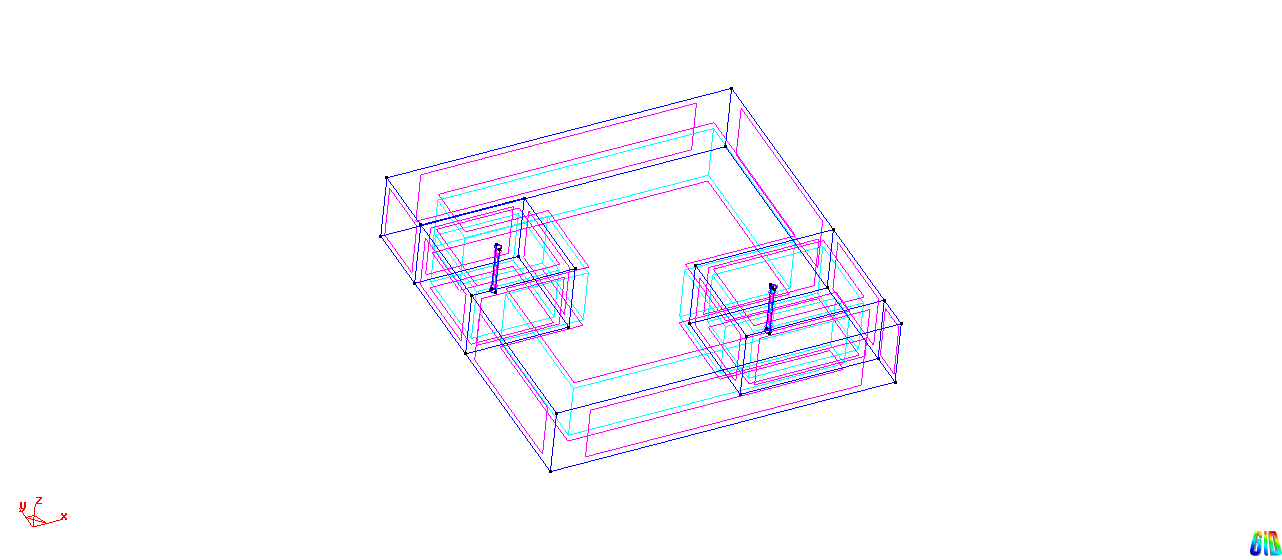
\includegraphics[scale=0.75]{img/superficies_y_volumenes}}
\caption{Superficies y Volúmenes de la Geometría}
\label{superficies_y_volumenes}
\end{figure}
%
%
%%
%\begin{figure}[tbhp]
%\centerline{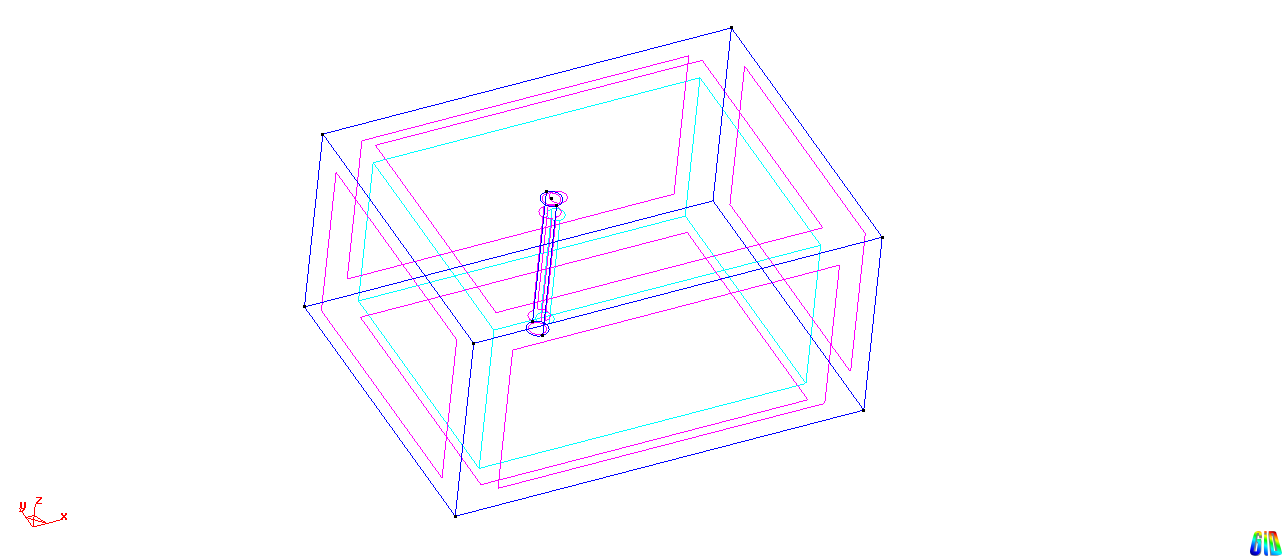
\includegraphics[scale=0.75]{img/detalle_pozo2_sup_vol}}
%\caption{Vista en detalle de las superficies y volúmenes generados (pozo 2)}
%\label{detalle_pozo2_sup_vol}
%\end{figure}
%%
%
%%
%\begin{figure}[tbhp]
%\centerline{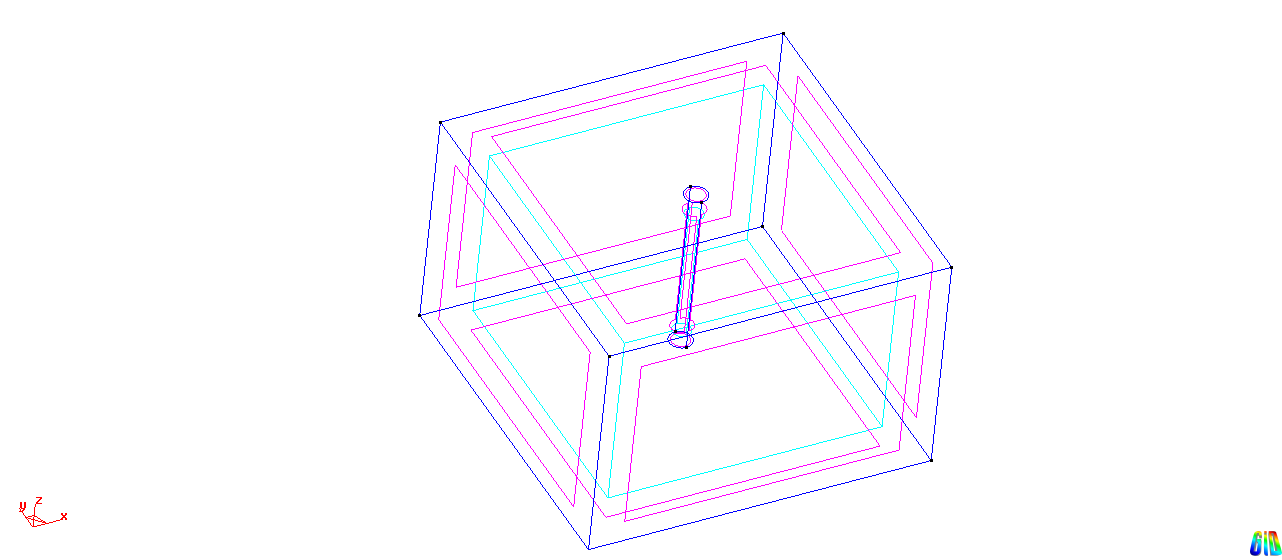
\includegraphics[scale=0.75]{img/detalle_pozo1_sup_vol}}
%\caption{Vista en detalle de las superficies y volúmenes generados (pozo 1)}
%\label{detalle_pozo1_sup_vol}
%\end{figure}
%%

%
\subsection{Propiedades del medio y de los materiales}
Características de Fluido: Flujo laminar, se comporta como viscoso por
la velocidad lenta.

%
\subsection{Condiciones de borde}
Condiciones de contorno: sacarlas del proyecto, enumerarlas y decir
que representa cada condición en nuestro problema. Recordar que
tenemos una condición que es la que calcula la función.
%
\subsection{Mallado}
contorno_malla_xy
contorno_malla_yz
%
\subsection{Condiciones temporales}
describir como oelegimos en
%
%
\subsection{Ejecución}
cambiar el titulo esto es como se llevo a cabao la corrida
%%%%%%%%%%%%%%%%%%%%%%%%%%%%%%%%%%%%%%%%%%%%%%%%%
%%%%%%%%%%%%%%%%%%%%%%%%%%%%%%%%%%%%%%%%%%%%%%%%%
%%%%%%%%%%%%%%%%%%%%%%%%%%%%%%%%%%%%%%%%%%%%%%%%%
\section{Resultados}
v(veloc) -> lineas de flujo/vect
p->equipotenciales
realizar cortes
%%%%%%%%%%%%%%%%%%%%%%%%%%%%%%%%%%%%%%%%%%%%%%%%%
%%%%%%%%%%%%%%%%%%%%%%%%%%%%%%%%%%%%%%%%%%%%%%%%%
%%%%%%%%%%%%%%%%%%%%%%%%%%%%%%%%%%%%%%%%%%%%%%%%%
\section{Conclusiones}
si el mod respondio
que problemas tuvimos? ahi hacer mencion al pozo grande y tiempo de calculo...
pozo real vs pozo simulado
%%%%%%%%%%%%%%%%%%%%%%%%%%%%%%%%%%%%%%%%%%%%%%%%%
%%%%%%%%%%%%%%%%%%%%%%%%%%%%%%%%%%%%%%%%%%%%%%%%%
%%%%%%%%%%%%%%%%%%%%%%%%%%%%%%%%%%%%%%%%%%%%%%%%%
\end{document}